\documentclass[output=paper]{langsci/langscibook} 
\author{Henning Radke\affiliation{Universiteit van Amsterdam}}
\title[The role of language contact in mixed-mode group communication]
      {The role of language contact in mixed-mode group communication: On ingroup construction through multilingualism among the German-Namibian diaspora}

\abstract{This paper analyzes the role of multilingual slang within mixed-mode groups through the example of the German Namibian diaspora. While digital single-mode groups only exist in computer-mediated communication (CMC), mixed-mode groups are involved in both CMC and face-to-face communication (FtF). This article focusses on the latter type of groups and addresses the question as to how contact-induced vernacular items are resemiotized from FtF to public and from spoken to written mode within these groups. It is hypothesized that the usage of multilingual slang in FtF mode and its corresponding group cohesion contribute to the frequency of slang within CMC. Furthermore, this study compares a mixed-mode group with a digital single-mode group to investigate the effects that the missing social contact within the latter group has on the tendency of its members to use multilingual slang in CMC. The German Namibian diaspora and their language practices are particularly suited to address this topic as they draw on multiple linguistic resources in their FtF and CMC networks with Afrikaans, German, and English being the main sources. In addition, Namibia’s multilingual setting has led to the emergence of a German-based variety, commonly referred to as   {Namdeutsch}. The resulting, multilingual practices are highly in-group specific. The study includes a mixed-method approach combining traditional FtF participant observation and modern correlation analysis of CMC data. The aim of this study is not only to shed light on the role of multilingual speech within mixed-mode groups. It also strives to contribute to the understanding of the complex dynamics that occur within diasporic settings. While recognizing the need for multiparadigmaticity in sociological and linguistic theory, this study stresses the importance of holistic approaches to analyze and understand language in social contexts because complex systems like diasporic groups are always more than just the sum of their component parts. In that sense, multilingual language practices are considered the result of diachronic and synchronic social interaction. }

\IfFileExists{../localcommands.tex}{
  % add all extra packages you need to load to this file

\usepackage{tabularx,multicol}
\usepackage{url}
\urlstyle{same}

\usepackage{listings}
\lstset{basicstyle=\ttfamily,tabsize=2,breaklines=true}

\usepackage{langsci-optional}
\usepackage{langsci-lgr}
\usepackage{langsci-gb4e}
% \usepackage{langsci-plots}
\usepackage{pgfplots}

\usepackage{siunitx}
\sisetup{group-digits=false}

\usepackage{amssymb}% http://ctan.org/pkg/amssymb
\usepackage{pifont}% http://ctan.org/pkg/pifont
\newcommand{\cmark}{\ding{51}}%
\newcommand{\xmark}{\ding{55}}%
% \usepackage[disable]{todonotes}
\usepackage{todonotes}

  \newcommand*{\orcid}{}
\newcommand{\hoederN}{n̡} 
  %% hyphenation points for line breaks
%% Normally, automatic hyphenation in LaTeX is very good
%% If a word is mis-hyphenated, add it to this file
%%
%% add information to TeX file before \begin{document} with:
%% %% hyphenation points for line breaks
%% Normally, automatic hyphenation in LaTeX is very good
%% If a word is mis-hyphenated, add it to this file
%%
%% add information to TeX file before \begin{document} with:
%% %% hyphenation points for line breaks
%% Normally, automatic hyphenation in LaTeX is very good
%% If a word is mis-hyphenated, add it to this file
%%
%% add information to TeX file before \begin{document} with:
%% \include{localhyphenation}
\hyphenation{
affri-ca-te
affri-ca-tes 
}
\hyphenation{
affri-ca-te
affri-ca-tes 
}
\hyphenation{
affri-ca-te
affri-ca-tes 
} 
  \togglepaper[1]%%chapternumber
}{}

\begin{document}
\maketitle 


 
\section{Introduction}
\label{sec:radke:1}

“In a 1973 lecture Dr. Paul Brandes of the University of North Carolina speculated that a link might exist between the internal cohesion of a group and the slang, or “in-group speech”, that the group evolves” \citep[55]{weinberg_measurement_1979}. Subsequently, Brandes and his colleagues set up a research project which eventually proved that this assumption was true. As a result, they developed the Group Cohesion Checklist (GROCC), a “tool for the measurement of cohesion and its slang through the investigation of group slang” \citep[55]{weinberg_measurement_1979}. Ever since, the idea that slang provides a means for groups to function in unity has constantly reappeared, especially in the field of sociology. “\citet{eble_slang_1996} stresses […] its function ‘to establish and reinforce social identity or cohesiveness within a group’” (\citealt[4]{fasola_slang_2011}; cf. \citealt[11]{eble_slang_1996}). And \citet[32]{mattiello_introduction_2008} notes that “slang is ascribed the two opposite purposes of keeping insiders together and outsiders out” (cf. \citealt[4]{fasola_slang_2011}). In short, slang serves to express, strengthen and maintain group cohesion, a phenomenon that \citet[55]{weinberg_measurement_1979} defines as “the unifying force of group syntality”.

However, since the GROCC was established in the 1970s, society has significantly changed, and new types of social groups have emerged. Due to the evolution of new media, many social groups of today choose to communicate within two different sorts of modes: the traditional \textit{face-to-face} mode (FtF) is one of them; computer-mediated communication (CMC) being the other, alternative mode with a profound influence on society. Groups of today can therefore be classified according to the mode(s) they use: while mixed-mode groups use both FtF communication and CMC, digital single-mode groups exclusively communicate in CMC and do not meet FtF.\footnote{Groups that exclusively communicate in FtF mode can also be referred to as single-mode groups. However, since the digitalization is constantly increasing on a global scale this type of single-mode group is becoming rare.}  This development leads to the following question: to what extent do linguistic habits in FtF affect CMC-based speech within mixed-mode groups? This article addresses this question through the example of the German-Namibian diaspora, e.g. German-speaking Namibians who migrated to Germany for study or work (cf. \citealt{radke_urban_inpress}). It is hypothesized that contact-induced vernacular items are resemiotized from FtF to public and from spoken to written mode when the mixed-mode group communicates in CMC. Thereby, these items are highlighted as ingroup identity markers, as illustrated in \tabref{tab:radke:1}.
 
\begin{table}
\begin{tabularx}{0.87\textwidth}{ccc}
\lsptoprule
\multicolumn{3}{c}{mixed-mode groups (in language-contact settings)}\\
\hline
${\Downarrow}$ & & ${\Downarrow}$ \\
face-to-face mode & ${\Leftrightarrow}$ & {CMC mode}\\
${\Downarrow}$ & resemiotization & ${\Downarrow}$ \\
 high slang frequency & & high slang frequency\\
(identity marker) & & (identity marker) \\
\lspbottomrule
\end{tabularx}
\caption{The hypothesized dynamics between different modes in mixed-mode groups.}
\label{tab:radke:1}
\end{table}  



The German-Namibian diaspora and their linguistic output in computer-mediated communication are particularly suited to empirically apply the given model, as they meet all necessary requirements: they have established a mixed-mode group named \textit{NAMSA}\footnote{NAMSA is an acronym for \textbf{\textit{Nam}}\textit{ibia} and \textbf{\textit{S}}\textit{üd}\textbf{\textit{a}}\textit{frika}. Up until Namibian independence in 1990, the event was known as SWASA, an acronym for \textbf{\textit{S}}\textit{üd}\textbf{\textit{w}}\textit{est-Afrika} and \textbf{\textit{S}}\textit{üd}\textbf{\textit{a}}\textit{frika}.}, as well as a single-mode group by the name of \textit{Namibianer} \textit{in} \textit{Deutschland} \textit{(NiD)} to maintain their Networks of Exchange (NoE).\footnote{See \citetv{chapters/08_Rocker} on East Frisians in Pennsylvania and their correspondences in a German newspaper for a historic example of a German-speaking minority using written media and communication to maintain a sense of belonging and identity.} Although, this article focuses on mixed-mode communication, \sectref{sec:radke:4} draws a comparison between both types of groups. It is expected that NiD deploys a less frequent degree of multilingual slang due to the lack social contact within FtF settings and a potentially lower degree of social group cohesion. Therefore, the language use in NiD is expected to be more standard-oriented and to lack slang items and traces of language contact.%\footnote{See Rocker (this volume) on East Frisians in Pennsylvania and their correspondences in a German newspaper for a historic example of a German-speaking minority using written media and communication to maintain a sense of belonging and identity.} Although, this article focuses on mixed-mode communication, \sectref{sec:radke:4} draws a comparison between both types of groups. It is expected that NiD deploys a less frequent degree of multilingual slang due to the lack social contact within FtF settings and a potentially lower degree of social group cohesion. Therefore, the language use in NiD is expected to be more standard-oriented and to lack slang items and traces of language contact.

The German-Namibian diaspora draws their slang from multilingual settings, with Afrikaans, German and English as the main source languages. As a result, German Namibians have developed a wide range of Namibia-specific language practices ranging from ad-hoc borrowings and code-switching/mixing to Namdeutsch (\citealt{bohm_deutsch_2003}; \citealt{duck_namibia_2018}; \citealt{gretschel_status_1995}; \citealt{kellermeier-rehbein_namslang_2015, kellermeier-rehbein_sprache_2016}; \citealt{nockler_sprachmischung_1963}; \citealt{putz_sudwesterdeutsch_1991}; \citealt{wiese_deutsch_2014, wiese_german_2017}; \citealt{wiese_registerdifferenzierung_2021}; \citealt{zimmer_deutsch_2019}). 
\citetv{chapters/05_Bracke} shows that younger speaker tend to use \textit{Namdeutsch} more frequently than older speakers while gender has not a clear effect on the speaker’s tendency to use Namibia-specific characteristics in their speech. Kellermeier-Rehbein uses the term \textit{Namslang} to denote Namdeutsch and defines it as „eine durch Sprachkontakt entstandene Nonstandardvarietät der deutschen Sprache in Namibia, die durch zahlreiche Entlehnungen von sprachlichen Einheiten und Strukturen aus dem Englischen und Afrikaans gekennzeichnet ist“ („A non-standard variety of the German language in Namibia created through language contact, which is characterized by numerous borrowing of language units and structures from English and Afrikaans“) (\citealt[228]{kellermeier-rehbein_sprache_2016}; cf. \citealt{radke_urban_inpress}). Stuhl \citetv{chapters/04_Stuhl} argues that \textit{Namdeutsch} is phonetically similar to Northern German and bases her findings on the analysis of two characteristic vowels and four consonants.\todo{this vol} %Stuhl (this volume) argues that \textit{Namdeutsch} is phonetically similar to Northern German and bases her findings on the analysis of two characteristic vowels and four consonants.%Bracke (this volume) shows that younger speaker tend to use \textit{Namdeutsch} more frequently than older speakers while gender has not a clear effect on the speaker’s tendency to use Namibia-specific characteristics in their speech. Kellermeier-Rehbein uses the term \textit{Namslang} to denote Namdeutsch and defines it as „eine durch Sprachkontakt entstandene Nonstandardvarietät der deutschen Sprache in Namibia, die durch zahlreiche Entlehnungen von sprachlichen Einheiten und Strukturen aus dem Englischen und Afrikaans gekennzeichnet ist“ („A non-standard variety of the German language in Namibia created through language contact, which is characterized by numerous borrowing of language units and structures from English and Afrikaans“) (\citealt[228]{kellermeier-rehbein_sprache_2016}; cf. \citealt{radke_urban_inpress}). Stuhl \citetv{chapters/04_Stuhl} argues that \textit{Namdeutsch} is phonetically similar to Northern German and bases her findings on the analysis of two characteristic vowels and four consonants.\todo{this vol} %Stuhl (this volume) argues that \textit{Namdeutsch} is phonetically similar to Northern German and bases her findings on the analysis of two characteristic vowels and four consonants.

In the given diasporic setting, Namibia-specific language practices are considered a form of slang. \citet[634]{lantto_code-switching_2014} cites “Andersson and Trudgill (1990:82–84) [who] suggest that slang can be created by inventing new expressions, by changing the old ones and by borrowing.” Then Lantto continues: “I would add code-switching to this list” \citeyear[634]{lantto_code-switching_2014}. The current article draws on the broad definition proposed by Lantto and thus considers the full range of Namibia-specific language practices. 

Hence, the German-Namibian diaspora is seen as a multilingual speech community that uses community-specific language practices rather than separate language systems. To give three examples: first, metrolingualism, which stresses linguistic fluidity in urban settings (\citealt{otsuji_metrolingualism:_2010}). Second, the notion of networked multilingualism, which “encompasses everything language users do with the entire range of linguistic resources within three sets of constraints: mediation of written language by digital technologies, access to network resources, and orientation to networked audiences” (\citealt[185]{androutsopoulos_networked_2015}; \citealt{radke_urban_inpress}). 

The third example refers to the diasystematic construction grammar or DCxG. It “assumes that multilingual speakers and communities organise their grammatical knowledge on the basis of the available input […] regardless of language boundaries” \citep[2]{hoder_grammar_2018}. Therefore, DCxG provides a means to analyze linguistically hybrid forms, amongst others (cf. \citealt[23]{hoder_mehrsprachige_2018}). \REF{ex:radke:1} shows an example of such a form taken from German Namibian CMC.

%%1st subexample: change \ea\label{...} to \ea\label{...}\ea; remove \z  
%%further subexamples: change \ea to \ex; remove \z  
%%last subexample: change \z to \z\z 

\ea
\label{ex:radke:1}
	\ea \label{ex:radke:1a} Original: a\textbf{g} nee 
	\ex \label{ex:radke:1b} German: a\textbf{ch} nee
	\ex \label{ex:radke:1c} Afrikaans: a\textbf{g}
	\ex \label{ex:radke:1d} English: I see
\z
\z

From a DCxG perspective, the frame of the chunk is a language-unspecific diaconstruction, including a language-specific idioconstruction, that is <ch> for German and <g> for Afrikaans. Both variants exist in German Namibian CMC. They clearly indicate the language of origin, as they are subject to language-specific spelling conventions. For this reason, DCxG refers to them as language markers \citep[23]{hoder_mehrsprachige_2018}. More specifically, \REF{ex:radke:1} contains a graphematic language marker since it does not imply phonetic but rather graphematic variation. An DCxG analysis of these hybrid forms is provided in \REF{ex:radke:2}.

\ea
\label{ex:radke:2}
 	\ea \label{ex:radke:2a} 
 	Partially Schematic Diaconstruction: {[}a\_\_c\textit{\textsubscript{ch,} \textit{g}}\textsubscript{} nee ‚I see’{]}
	\ex \label{ex:radke:2b}
 	Graphematic Language Marker: {[}C\textsubscript{(}\textit{\textsubscript{ch,} \textit{g:} \textit{g}}\textsubscript{)} $\langle$C\textsubscript{afrikaans}$\rangle${]}
	\ex\label{ex:radke:}
 	Graphematic Language Marker:{[}C\textsubscript{(}\textit{\textsubscript{ch,} \textit{g:} \textit{ch}}\textsubscript{)} $\langle$C\textsubscript{german}$\rangle$〉{]} 
\z
\z

\REF{ex:radke:2} shows how the multilingual setting of Namibia is reflected in hybrid forms on a graphematic level. The component \_\_c\textsubscript{ch, g}   {indicates a consonant space which can orthographically either be filled with <ch> or <g> (see \citealt[16]{hoder_mehrsprachige_2018}). It shows that both variants} ach nee   {and} ag nee   {coexist in German Namibian CMC.}\footnote{There are several other hybrid pairs used in German Namibian CMC that can be analyzed in the same way, e.g. \textit{a}\textbf{\textit{ch}}\textit{so/a}\textbf{\textit{g}}\textit{so,} \textit{Jun}\textbf{\textit{i}}\textit{/Jun}\textbf{\textit{ie}}, \textit{Mus}\textbf{\textit{i}}\textit{k/mus}\textbf{\textit{ie}}\textit{k,} \textit{bis} \textit{da}\textbf{\textit{nn}}\textit{/bis} \textit{da}\textbf{\textit{n}}, \textit{na} \textit{kl}\textbf{\textit{a}}\textit{r/na} \textit{kl}\textbf{\textit{aa}}\textit{r}.}  The variation between them can, therefore, be considered a community-specific practice within the German-Namibian diaspora and is part of what Höder describes as a cross-language constructional network (“[…] des sprachübergreifenden konstruktionellen Netzwerks”) of a multilingual community (see \citealt[15]{hoder_mehrsprachige_2018}).\footnote{For an in-depth analysis on the constructional perspective and its role in analyzing  grammatical arealisms in Danish and German, see \citetv{chapters/02_Hoeder}.}\\%\footnote{For an in-depth analysis on the constructional perspective and its role in analyzing  grammatical arealisms in Danish and German, see Höder (this volume).}\\
The German-Namibian diaspora thus combines all necessary preconditions to test the given model outlined in \tabref{tab:radke:1}. In doing so, I have conducted research at the interface of sociology, social psychology and sociolinguistics. The common epistemological interest of these disciplines focuses on the relationships between individuals and groups in social interaction. Sociology aims to explain human behavior through structural variables such as social norms and roles, whereas social psychology rather focuses on inner processes of the human mind, e.g. goals and attitudes (cf. \citealt[11]{jonas_sozialpsychologie_2014}). This paper combines both perspectives to shed more light on the role and function of language in society through the example of the German-Namibian community. In doing so, it builds a bridge to the field of sociolinguistics.

 
\section{Methodology}
\label{sec:radke:2}
 

Not surprisingly, a study of mixed-mode groups requires a mixed-method approach, considering both FtF and CMC data. I therefore chose to combine FtF-based participant observation with correlation analysis of CMC data originating from the same group. Participant observation was conducted during the annual three-day NAMSA event in June 2019. It included direct observation, collective discussions, and participation in the activities of the group. These methods are part of the \textit{participant} \textit{as} \textit{observer} role, which is one of the four major roles identified by Raymond \citet{gold_roles_1958} and Buford \citet{junker_field_1960}.\footnote{See also \url{https://www.encyclopedia.com/social-sciences-and-law/sociology-and-social-reform/sociology-general-terms-and-concepts-87} [8 November 2019].} It also includes that respondents are aware of the research being conducted. This approach “may be considered moderate participation by Spradley” (\citealt{howell_preparing_2018}:211; cf. \citealt[58]{spradley_participant_1980}), with its main objective to maintain “a balance between ‘insider’ and ‘outsider’ roles that allows a good combination of involvement and necessary detachment to remain objective” (\citealt[211]{howell_preparing_2018}; cf. \citealt[58]{spradley_participant_1980}). Since NAMSA is an ingroup event par excellence, it was possible to obtain a genuine impression of ingroup speech practices, e.g. the usage of diasporic Namdeutsch. 

However, participant observation bears the risk of collecting data with a subjective bias. For this reason, the applicability of my analysis was evaluated based on a three-fold process: by member-checking, by participatory peer-reviewing and by non-participatory peer-reviewing. Member-checking included the feedback of German-Namibians on the descriptive validity of \sectref{sec:radke:3}. Participatory peer-reviewing included the feedback of a fellow outgroup member with profound knowledge of Namibian cultures and who was present during participant observation.\footnote{Many thanks to Merrick Nock for his feedback.} Non-participatory peer-reviewing included the feedback of fellow (socio-)linguists during three conferences in Berlin, Hanover and Göttingen.\footnote{Many thanks to Prof. Horst Simon and Dr. Christian Zimmer for inviting me to deliver a talk during the conference \textit{German(ic)} \textit{in} \textit{language} \textit{contact:} \textit{Grammatical} \textit{and} \textit{sociolinguistic} \textit{dynamics} (Berlin, 3--5 July 2019) and the \textit{Sommerkolloquium} (Hanover, 12--14 July 2019). Furthermore, I owe many thanks to Klaus A. Hess and the \textit{Deutsch-Namibische} \textit{Gesellschaft} \textit{e.V.} for inviting me to speak at their \textit{Wochenendseminar} (Göttingen, Germany, 27 October 2019).} These member checks aim to enhance the internal validity of the collected data and the analysis presented in this paper.

Not surprisingly, FtF-based participant observation could only be conducted for NAMSA, as NiD is a CMC-only group with no FtF-platform. However, the application of correlation analysis to CMC data covered both groups, pointing out the importance of a mixed-method approach for this study (see \sectref{sec:radke:4.2}). The CMC data originate from social media and cover the linguistic output within NAMSA and NiD, as well as the sociodemographic metadata of their users, such as place of origin, place of residence and gender. The data were automatically exported to a spreadsheet using the add-on programme \textit{Web} \textit{Scraper}. Subsequently, the linguistic output could be annotated and correlated to the corresponding sociodemographic metadata. The resulting corpus consists of 2,178 comments: 67\% or 1,451 comments were exclusively published in Standard German whereas 33\% or 727 comments include Namibia-specific language practices on the orthographic, lexical or morphosyntactic level (see \citealt{radke_urban_inpress}).

This study thus combines traditional methods with new approaches to collect and analyze data. Participant observation was formalized in the 1950s, whereas CMC-based correlation analysis has gained significant importance in recent years. The mixed-method approach not only allows for a description of trans-national networks within the German-Namibian community, it also sheds more light on the dynamics within mixed-mode groups and on the role of slang for the formation of ingroups and outgroups (\sectref{sec:radke:3.2}). First, I will turn to the findings made during participant observation (\sectref{sec:radke:3.1} and \sectref{sec:radke:3.2}). 

 
 \section{The Dynamics of a Mixed-Mode Group} 
 \label{sec:radke:3}

 
\subsection{FtF Communication within NAMSA}
 \label{sec:radke:3.1}
 

In this section, I will address the model outlined in \figref{fig:radke:1} to lay bare the multilingual dynamics within the mixed-mode group of NAMSA. It is hypothesized that contact-induced vernacular items are resemiotized from FtF to public and from spoken to written mode when the group communicates in CMC. Thereby, these items are highlighted as ingroup identity markers and frequently reoccur in CMC. The following figure shows the interplay between FfF and CMC. It also addresses the linguistic behavior of ingroup members and its social psychological and sociological parameters. 

  
%%please move the includegraphics inside the {figure} environment
%%
 

\begin{sidewaysfigure}
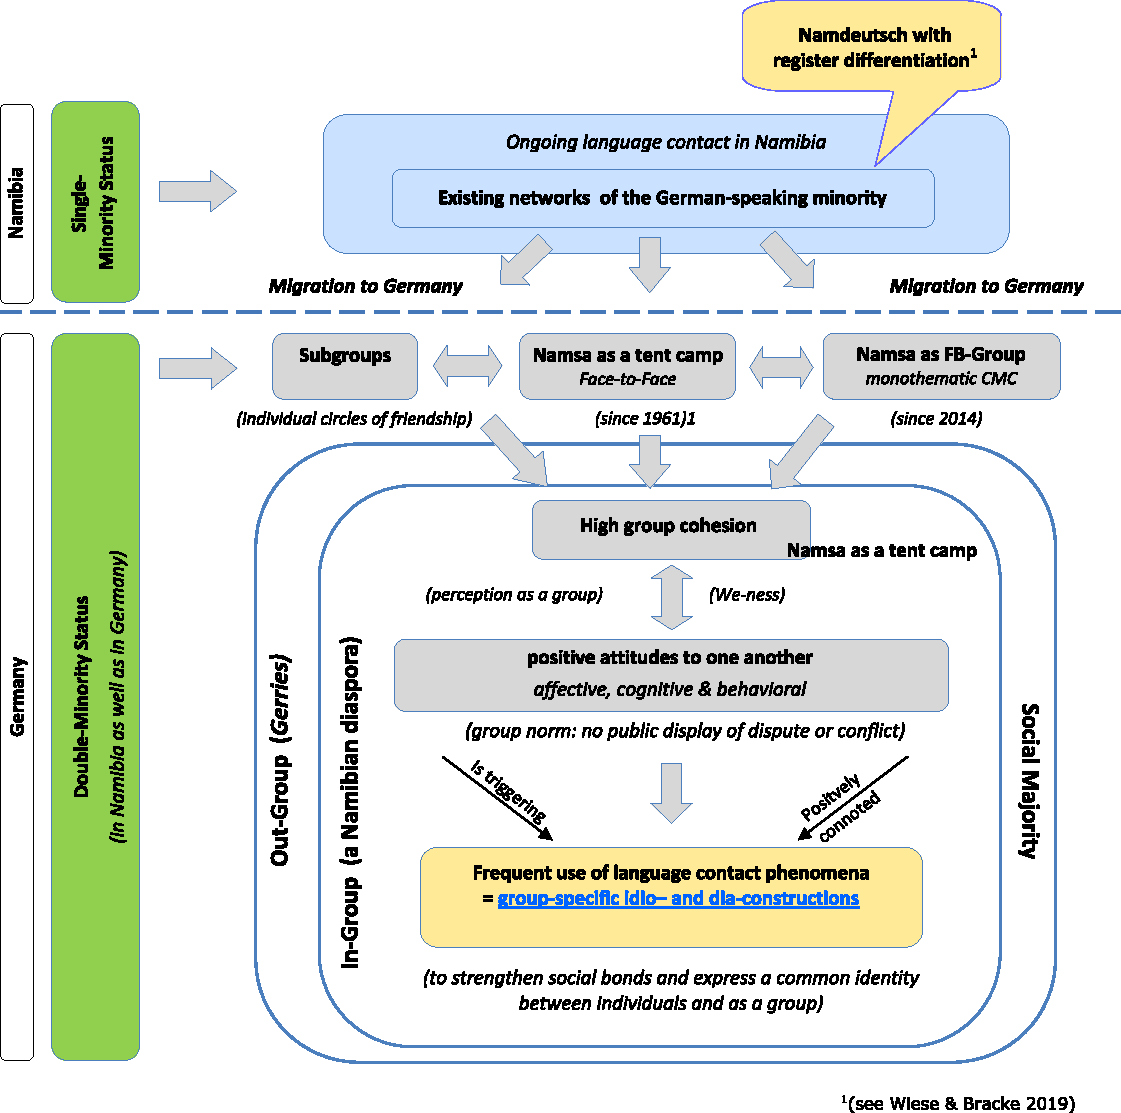
\includegraphics[width=0.8\textwidth]{figures/radkefig1-carla.pdf}
\caption{The social context of Namdeutsch}
\label{fig:radke:1}
\end{sidewaysfigure}  

\figref{
} shows that the transnational networks of German Namibians are based in an ongoing language contact situation in Sub-Saharan Africa. Besides Namibia, they extend across several other countries with Germany and South Africa being the main destinations for the German Namibian diaspora. The most influential contact languages are Afrikaans and English; indigenous languages of Namibia have had limited influence on their ingroup speech (\citealt{bohm_deutsch_2003}; \citealt{duck_namibia_2018}; \citealt{kellermeier-rehbein_namslang_2015, kellermeier-rehbein_sprache_2016}; \citealt{nockler_sprachmischung_1963}; \citealt{putz_sudwesterdeutsch_1991}; \citealt{wiese_deutsch_2014, wiese_german_2017, wiese_registerdifferenzierung_2021}; \citealt{zimmer_linguisticvar_toappear}; \citealt{zimmer_korpus_2020}). The sustainable language contact has led to the evolution of the vernacular \textit{Namdeutsch}. Trans-national networks between Germany and Namibia were formalized in the early 1960s by an initiative of Rosemarie Bernhardt, a young German Namibian who established the annual SWASA event (since 1990: NAMSA) during Pentecost (cf. \citealt{radke_afrikaans_2019a}). In the first decade of its existence, the network was maintained by letter mail. With the rise of CMC, the communication and the organization of NAMSA became digitized, first through its own forum and later on social media. In 2014, a digital NAMSA group was established on Facebook, reaching the landmark of 1,300 members five years later. Thus, NAMSA started as a single-mode group in the 1960s for mostly young Namibians, supported by postcard communication, and transformed into a mixed-mode group some 40 years later. 

Due to technological progress, the CMC-mode has gradually gained importance for the NAMSA group (\citealt{radke_urban_inpress}). Both FtF communication and CMC contribute to the development of social group cohesion, especially during the annual NAMSA event. There, members develop, maintain and deepen their sense of ‘we-ness’ and belonging to the group as a whole. They deploy a positive attitude towards one another, which is expressed in their affective, behavioral, and cognitive manners: they expect to meet old friends, make new ones, have a good time and exchange thoughts about Namibia-related topics in the middle of Germany. These expectations are central to their cognition. They are either based on prior experiences at NAMSA or created through story-telling of friends and acquaintances and mediated through social media. Cognition and affection interact with each other and so most participants expressed feelings of pleasant anticipation and joy when talking about (the upcoming edition of) NAMSA. Whoever they meet during the event will most likely be an ingroup member and will be treated as such. A positive attitude is shared by the overwhelming majority of the group members and leads to a central group norm, implying that public display of dispute or conflict is not welcomed. At least some of the group members explicitly referred to this norm, which they greet with approval. Consequently, behavior violating the norm meets disapproval by other members, in FtF communication as well as in CMC. Although the multilingual inventory for polemic language use is at their disposal (especially in Afrikaans with its descriptive compounds and phrasemes), ingroup members hardly ever use it in public FtF settings and CMC.\footnote{This observation does not necessarily mean that the \textit{no-conflict} norm also privately applies to all individual circles of friendships linked to the group at any given time.}

The aforementioned environment provides an ideal setting to trigger the use of language contact phenomena or Namibia-specific language practices, such as code-switching, ad-hoc borrowing and the use of Namdeutsch to strengthen social bonds and express a common identity between group members and the group as a whole. Key slang words reflect the construction of an ingroup and outgroup on a linguistic level: the social majority in Germany is referred to as \textit{Gerries}, whereas ingroup members are often addressed as \textit{Oukies}. Both terms are a result of language contact in Namibia: \textit{Oukie} is an Afrikaans borrowing (see \sectref{sec:radke:3.4}), whereas \textit{Gerrie} has evolved from the English word \textit{German} during World War One.\footnote{\url{https://www.etymonline.com/word/Jerry} {[}29-06-2020{]}.}   

The dynamics of ingroup construction are further supported by the fact that the German-Namibian diaspora represents what I call a double minority: they amount to 1\% of the population in their home country and thus draw on existing networks that are relatively easy to survey. Upon arrival in Germany, many of them indeed speak the language of the social majority (at least in its standard form) and have a sense of \textit{German-ness}. However, they grew up in Sub-Saharan Africa, in a country with different societal, economic and environmental conditions. Hence, they are German-Namibians,\footnote{Or Namibian-Germans or German-speaking Namibians, depending on the individual perception of each ingroup member.}  but not German-Germans, which makes many of them feel different (to a greater or lesser degree) from the (perceived) social majority in Germany.\footnote{See the article ‘Integration mit besten Voraussetzungen’ written by Katharina Herrle in which she describes her feeling of being an \textit{Ausländer} \textit{ohne} \textit{Ausländerbonus} (a foreigner without the benefits of being one) when she first came to Germany (Informationsausschuss der Deutschen Evangelisch-Lutherischen Kirche in Namibia DELK 2016:66).} During collective discussions, respondents confirmed that they had felt foreign in the initial stages of their stay in Germany. Therefore, the double minority status promotes ingroup construction and, in fact, triggers the use of language contact phenomena. 

 
   
\subsection{Ingroup and Outgroup Communication}
  \label{sec:radke:3.2}
 

The following figure shows the typical characteristics of ingroup and outgroup communication that are maintained by the transnational networks of the German Namibians in both CMC and FtF settings. 

\begin{sidewaysfigure}
 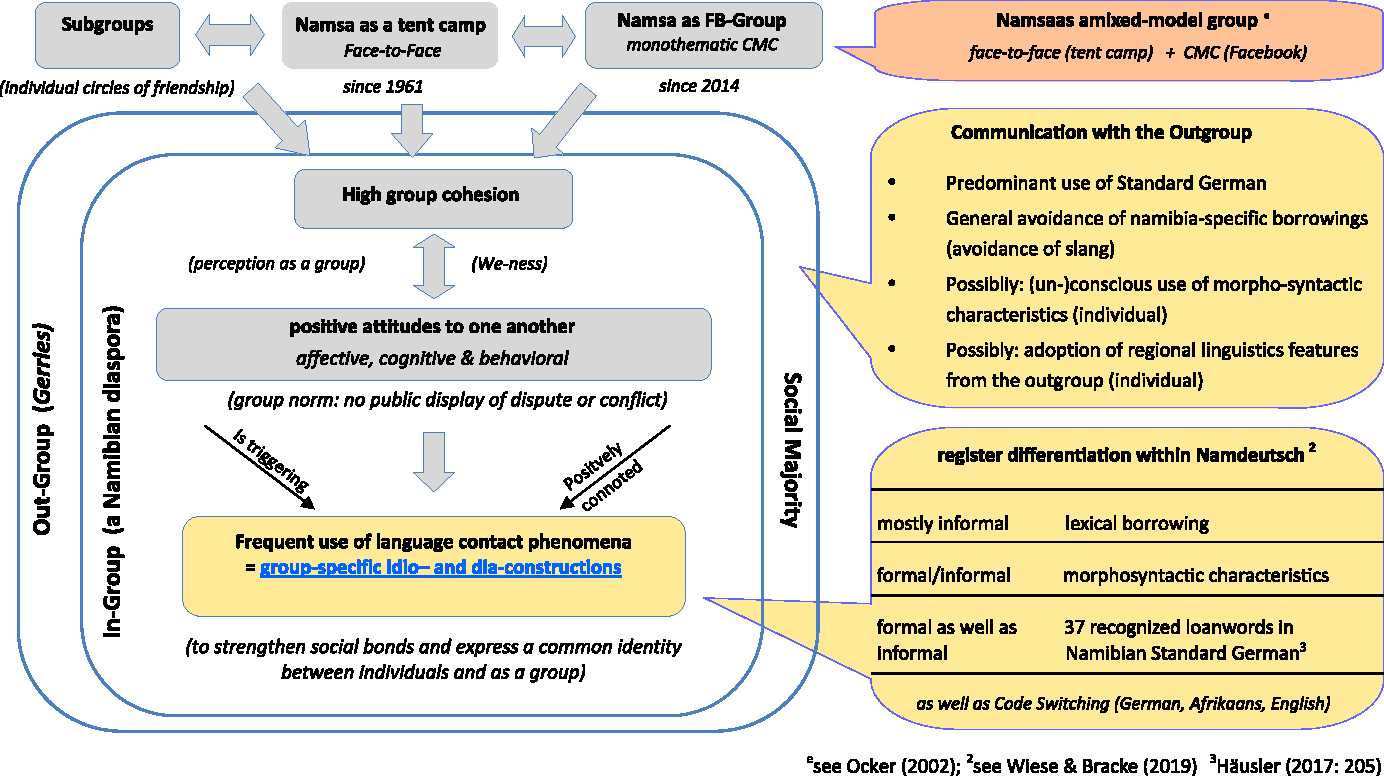
\includegraphics[width=0.9\textwidth]{figures/radkefig2-c.pdf}
\caption{Ingroup and Outgroup Communication}
\label{fig:radke:2}
\end{sidewaysfigure}  

The construction of an ingroup and an outgroup prompts two different linguistic styles among the community: ingroup communication features the frequent use of Namibia-specific language practices, whereas outgroup communication is predominantly characterized by Standard German and a (conscious) striving to avoid Namibia-specific language practices, e.g. slang. This observation applies to both lexical and morphosyntactic language choices. However, the latter is less accessible to human consciousness. Hence, during outgroup communication, the ingroup members are more likely to unconsciously use linguistic structures of Namibian origin other than lexical borrowings. However, awareness and use of such structures highly differ from individual to individual. 

To give an example: during the annual NAMSA event, an ingroup member talked to a local taxi driver on the telephone. Clearly, the driver was an outgroup member. So, the telephone call started off in Standard German until the moment when they both discussed the taxi prices. The ingroup member posed the following question:
\ea
\label{ex:radke:3}
 	\gll Wieviel \textbf{geht} das kosten? \\
		{how much}  go:\textsc{3sg;prs}   that  cost\textsc{:inf;prs}\\
     \glt `How much will it cost?'\\
 \z
 
\REF{ex:radke:3} shows the Namibia-typical use of the verb \textit{gehen} as a future marker.\footnote{This is probably due to language contact with Afrikaans and/or English (cf. \citealt[33]{shah_german_2007}; \citealt[234--35]{radke_hat_2019b})} In European German, a form of \textit{werden} (English: will) is the only auxiliary to mark the future tense.\footnote{\textit{werden}-future is the marked choice to indicate the future tense and includes an epistemic notion. The present tense is the unmarked choice and is often used when a temporal adverb or the context indicate future meaning instead. This applies to European and Namibian German.}  However, at the time of the telephone call, the ingroup member was not aware of the markedness that a \textit{gehen}-construction would have for his interlocutor. The use of this construction may have further been prompted by the Namibian character of the environment: the telephone call took place towards the end of NAMSA, making it likely that the ingroup member had been using Namibia-specific language practices for almost three days in a row. In other words, he was in a multilingual mode (cf. \citealt{hoder_mehrsprachige_2018}: 7), as everyone around him shared the same languages and he felt comfortable enough to join in (cf. \citealt[2]{grosjean_bilingual_2012}). The telephone call required a switch into the monolingual mode, which the ingroup member maintained on the lexical level. However, Namibia-specific language practices with a lesser degree of consciousness, such as tense marking, became reactivated due to the linguistic setting.
  
Unlike outgroup communication, ingroup discourses are characterized by the frequent use of Namdeutsch and Namibia-specific language practices, such as code-switching between German, Afrikaans, and English. Wiese and Bracke (in press) show that German-Namibians deploy different registers in Namdeutsch according to the level of formality of the communicative setting. Lexical borrowings are “stärker mit informellen Gesprächen assoziiert […], während das formelle Register nah am Standarddeutschen in Deutschland ist“ (Lexical borrowing is more associated with informal conversations, while the formal register is close to Standard German in Germany (\citealt[14]{wiese_registerdifferenzierung_2021}). However, even formal registers include Namibia-typical borrowings and grammatical patterns and indicate the existence of Namibian Standard German (\citealt{wiese_registerdifferenzierung_2021}). \citet{ammon_variantenworterbuch_2016} recognized 37 loanwords as being part of Namibian Standard German such as the onomasiological variants  \textit{Bakkie} (for \textit{Laster} = ‘pick-up truck’), \textit{Pad} (for   \textit{Weg}, \textit{Straße}  = ‘path’, ‘street’, ‘road’) and \textit{Permit}  (for \textit{Genehmigung}, \textit{Erlaubnis} = ‘permit’) or culture-specific terms such as \textit{Biltong} (dried meat),  \textit{Braai} (‘BBQ’) and \textit{Veld}   (a type of open and rural landscape in Southern Africa) \citep[206--207]{hausler_zur_2017}. One of the criteria for the terms to be recognized as Namibian Standard German was the frequent use in official language domains such as newspapers (2016). \figref{fig:radke:2} shows the dichotomy between ingroup and outgroup communication in relation to the sociological and social psychological dynamics of group formation for NAMSA. Therefore, it stresses the importance of a holistic perspective on ingroups to understand the dynamics that evolve through social interaction.
  

 
   
\subsection{Mixed-Modes and Group Cohesion}
 \label{sec:radke:3.3}
 

Since NAMSA provides a reoccurring platform for FtF communication, it is likely to positively affect the group cohesion among its members. The correlation between cohesion and FtF communication has been subject to only a few studies. \citet{ocker_mediating_2002} investigated the interplay between workgroup cohesion, conflict management, and satisfaction. These aspects can be considered key forces “causing members to remain in their group” (\citealt[246]{carron_development_1985}; \citealt[276]{brawley_assessing_1987}; cf. \citealt{festinger_social_1950}). According to Ocker, mixed-mode groups are more cohesive than single-mode groups.

\begin{quote}
Members of mixed-mode groups rated their groups higher in terms of cohesiveness, the ability to manage conflict, and all aspects of satisfaction. \citep[1]{ocker_mediating_2002}
\end{quote}

These findings provide a first hint that mixed-mode groups, in general, develop a higher degree of cohesion. However, it is important to carefully define this term. According to \citet[127]{shin_role_2011},  “cohesion is a multidimensional construct that encompasses both social and task aspects of the group process (cf. also \citealt[276]{brawley_assessing_1987}; \citealt{carron_development_1985}).

\begin{quote}
[…] social cohesion is defined as the degree to which an individual is attracted to the group because of his or her positive relationships with other group members. However, task cohesion refers to the degree to which an individual is attracted to the group because of his or her shared commitment to group tasks (\citealt[127]{shin_role_2011}; cf. \citealt[276]{brawley_assessing_1987})
\end{quote}

In this regard, too, mixed-mode groups have a higher potential to develop and maintain a coherent group feeling, as the two “different types of cohesion can be developed through different modes of communication or interaction” (\citealt[136]{shin_role_2011}). 

\begin{quote}
The findings suggest that time spent in FTF communication significantly predicted group social cohesion, but time spent in CMC did not. […] These results suggest that FTF communication contributes to the social aspect of mixed-mode groups and that CMC is beneficial to their task-related aspect. (\citealt[126]{shin_role_2011})
\end{quote}

What Shin and Song describe in their research, does also apply to NAMSA: here, CMC is predominantly used to organize an annual FtF meeting during Pentecost. Therefore, it serves to distribute information on location, time and other practical matters, and to welcome new members. Hence, NAMSA functions as a predominantly task-related CMC group with the main purpose of organizing an FtF event in which the social aspect of group cohesion is central.\footnote{Information on other practical matters, such as housing in Germany, is common as well. However, the main focus remains on the NAMSA event.} In this respect, the German Namibian diaspora combines both task- and social-related modes. However, in the (immediate) period after each NAMSA event, the CMC group also serves as a virtual platform for continuing experiences of the FtF setting: many members post photos taken during the event and subsequently comment on them. This way, members relate to the social aspect of the group process by bringing it up in CMC, as can be seen in \REF{ex:radke:4}. Namibia-specific language practices are highlighted in bold.\todo{original examples with emoji}


\ea\label{ex:radke:4}
	\ea Julia: \textit{Vielen Dank an alle für dieses herrliche Wochenende und das Stück Heimat-Feeling} \\
	
	Thanks a lot to everyone for the wonderful weekend. It gave me a feeling of home   

	\ex Britta: \textit{Das war \textbf{moois}}\\

	 It was nice
\z
\z
   
\subsection{NAMSA: Slang and Identity in CMC} 
  \label{sec:radke:3.4}
  
  \subsubsection{Afrikaans-based Keywords}
 \label{sec:radke:3.4.1}

Since the multilingual dynamics in FtF communication have been analyzed in \sectref{sec:radke:3.1}, I will now turn the focus on CMC-based language practices. The following question takes center stage: does multilingual slang serve as a marker for ingroup identity in CMC among the German Namibian diaspora? I will, therefore, draw on a corpus-based analysis of the 10 most frequently used keywords, all of which are borrowings from Afrikaans. To identify these keywords, I used an automated word frequency counter by Gillmeister Software.\footnote{\url{https://www.gillmeister-software.de/online-tools/text/keywortdichte-berechnen-fuer-seo.aspx} [23-06-2020]} The resulting list indicates all words (or word combinations) that exist in a given text corpus. Furthermore, it provides the absolute number of their occurrences. Subsequently, the list can be exported to a spreadsheet. The Afrikaans-based borrowings were manually lemmatized and orthographically harmonized. In doing so, all inflected forms and orthographic variants of a given word could be analyzed as a single item (e.g.: \textit{mooi,} \textit{moi,} \textit{mooie,} \textit{mooier,} \textit{mooies,} \textit{mooije,} \textit{mooin} were counted as \textit{mooi} = ‘beautiful’, ‘nice’). The resulting frequency list of Afrikaans-based keywords can be seen in \figref{fig:radke:3}.



  
%%please move the includegraphics inside the {figure} environment
%%\includegraphics[width=\textwidth]{figures/a06Radke-img006.svm}
 

  \begin{figure}
   \begin{tikzpicture}%[trim axis right,trim axis left]
    \begin{axis}[
        axis lines*=left,
        width  = {.99\textwidth},
        height  = {.33\textheight},
%         nodes near coords,
        xlabel style={xshift=0.5cm},
        x tick label style={rotate = 45},
        ytick = {0, 20, 40, 60, 80, 100, 120, 140},
         %ytick=data,
        ymajorgrids,
        bar width=.3cm,
        xmin=0,
        %legend style={at={(1,0.01)},anchor=south east},
        %reverse legend,
        nodes near coords,
        every node near coord/.append style={anchor=south},
        symbolic x coords={
        0,
        ou/oukie,
        net,
        mooi, 
        lekker, 
        bikkie, 
        kak, 
        plek/plekke, 
        jerre/jirre, 
        mos, 
        gees}
        ]
        \addplot[ybar,silptwo!80!black,fill=silptwo] plot coordinates {
        (ou/oukie, 122)
        (net, 99)
        (mooi, 80)
        (lekker, 72)
        (bikkie, 54)
        (kak, 39)
        (plek/plekke, 35)
        (jerre/jirre, 30)
        (mos, 30)
        (gees, 21)
            };
        %\legend{Year 1, Year 3}
    \end{axis}
\end{tikzpicture}
\caption{Afrikaans-based keywords in German-Namibian CMC. \textit{ou/oukie(s)} = ‘dude(s)’, ‘mate(s)’, ‘guy(s)’; \textit{net} = ‘only’; \textit{mooi} = ‘beautiful’, ‘nice’; \textit{lekker} = ‘delicious’, ‘pleasant’, ‘nice’; \textit{bikkie} = ‘a bit’; \textit{kak} = ‘shit’; \textit{plek/plekke} = ‘place(s)’, ‘venue(s)’; \textit{jerre/jirre} = ‘interjection’; \textit{mos} = modal particle; \textit{gees} = ‘mood’}
\label{fig:radke:3}
\end{figure}  

The list of keywords contains four categories of borrowings: first, the interjection \textit{jirre/jerre} and the modal particle \textit{mos.} Both are typical signs of orality which is in line with CMC seen as a written form close to  spoken language. Furthermore, they can be used for appellative and expressive purposes, such as in \REF{ex:radke:5} and \REF{ex:radke:6}

\ea
\label{ex:radke:5}
\gll \textbf{Jerre} oukie hast du dich erst jetzt von Namsa erholt? \\
	Wow oukie have you yourself only now of NAMSA recovered?\\
	\glt `Wow oukie, have you only just recovered from NAMSA?'\\
\z


\ea
\label{ex:radke:6}
\gll aber hey wir \textbf{liken} das Leben \textbf{mos} bunt!\\
   But hey, we like the life \textsc{part}  colorful\\
\glt  `But hey, after all we like it when life is colorful.'\\
\z

The second category includes the adjectives \textit{mooi} (‘beautiful’, ‘nice’) and \textit{lekker} (‘delicious’, ‘pleasant’, ‘nice’), which are used to express politeness, reassurance and a positive attitude towards one another. Third, the downtoners \textit{bikkie} (‘a bit’) and \textit{net} (‘just’, ‘only’) serve to reduce the force of another word or phrase. Therefore, they too are often part of politeness strategies. And fourth, the three most frequently used nouns of Afrikaans origin are \textit{ou/oukie} (‘dude’), \textit{gees} (‘mood’) and \textit{plek/plekke} (‘venue’/’venues’). \textit{Ou/oukie} and \textit{gees} often serve to address other users and to prompt positive reactions, as can be seen in \REF{ex:radke:7} and \REF{ex:radke:8}:

\ea
\label{ex:radke:7}
 \gll \textbf{Lecker} man. Bringt alle \textbf{stief} \textbf{gees} mit! \\
   		Delicious man bring all much mood with\\
     	\glt `Great, man. Bring good vibes with you!'\\
\z


\ea\label{ex:radke:8}
	\gll Mark hat \textbf{gees} heute \\
		Mark has mood today\\
     \glt `Mark is keen today.' \\
\z
 
\textit{Plek/plekke} is an exceptional case among the most frequent keywords, as it does not bear any expressive or appellative meaning in itself. Its frequency is rather caused by the monothematic setup of NAMSA, in which members often discuss suitable venues to hold the FtF event. To indicate the concept of “venue”, users often use the Afrikaans word \textit{plek/plekke}. Another exceptional keyword is the pejorative \textit{kak} (‘shit’), since it bears a derogatory meaning that potentially violates the norms of individuals and groups. However, \textit{kak} is not used in an offensive way towards other members in the first place, but rather serves as a descriptive or expressive intensifier. In that respect, it does not seem to violate any norm within German Namibian CMC, as can be seen in \REF{ex:radke:9} and \REF{ex:radke:10}:

\ea\label{ex:radke:9}
	\gll Mal abwarten […] weil die Verbindung ist \textbf{Kak}\\
		Once wait […] because the connection is shit.\\
	\glt `Let’s wait because the connection is bad.'\\
\z

\ea\label{ex:radke:10}
	\gll Ohne \textbf{Kak}? Jerre nice welche Daten? \\
		Without shit wow nice which dates\\
	\glt `Seriously? Wow, nice. Which dates?'\\
\z

Although \textit{kak} is a term of disparagement, it is predominantly used in a neutral way. Therefore, it does not counteract the functions of the aforementioned keywords, all of which are mostly used for appellative and expressive purposes to show a positive attitude towards the group. However, do these multilingual keywords also serve to construct ingroups and outgroups? To answer this question, I will turn to the most frequently used keyword in German-Namibian CMC: the term \textit{ou/oukie.} As a singular noun it refers to a male person (‘dude’, ‘mate’, ’guy’) whereas the plural form \textit{oukies} can be used as a gender-neutral term in the sense of ‘(you) guys’. In 3.4.2., I will examine whether is it used to create linguistic identities and, hence, a notion of inclusiveness versus exclusiveness in German Namibian CMC.

 
  \subsubsection{Inclusiveness versus Exclusiveness}
 \label{sec:radke:3.4.2}

“Linguistic identities are double-edged swords because, while functioning in a positive and productive way to give people a sense of belonging, they do so by defining an ‘us’ in opposition to a ‘them’” \citep[261]{joseph_linguistic_2006}. The construction of such an ‘us‘ versus a ‘them’ through Namibia-specific language practices is shown in \REF{ex:radke:11}--\REF{ex:radke:13}.
\ea
\label{ex:radke:11}
Dennoch hier noch mal an die Frage erinnert, ob wir hier auch \textbf{oukies} \textbf{und} \textbf{ladies} in Berlin haben :-)Vielleicht sucht ja auch jemand ein Zimmer in Berlin, während der Zeit, in der ich unten bin [in Namibia].\\
\textit{Still, coming back to the question of whether there are also} \textbf{oukies} \textbf{and} \textbf{ladies} in Berlin :-) Maybe someone is looking for a room in Berlin when I‘m down there [in Namibia].\\
\z

\ea\label{ex:radke:12}
ein paar \textbf{Oukies} aus München haben die \textbf{Gees} und organizen es dieses Jahr ... Für Euch nicht \textbf{Gerries}\\
\textit{A few \textbf{oukies} from Munich are keen and will organize it this year... Not for you, \textbf{Gerries}}.\\
\z

\ea\label{ex:radke:13}
 \textbf{Definitely}!!! \textbf{Oukies} kriegen nie genug...\\
\textit{{Definitely!!!} \textbf{{Oukies}} {can never get enough...}}\\
\z

\REF{ex:radke:11}--\REF{ex:radke:13} imply different levels of ingroup and outgroup construction through the use of Namibia-typical borrowings. In \REF{ex:radke:12}, a German Namibian user offers to sublet his room in Berlin, as he is planning an extended stay in Namibia. He wonders whether there are any \textit{oukies} \textit{und} \textit{ladies} who may be interested in his offer. In doing so, he indicates his preference to rent out his room to an ingroup member, that is to say a German Namibian. This practice bears a mutual advantage:  ingroup members in search of accommodation will find it easier to get a room. In addition, the advertiser may perceive it as safer to rent out his personal space to a person of the same network. Hence, the term \textit{oukies} \textit{und} \textit{ladies} addresses German Namibians in Berlin, as opposed to any other individual who is looking for accommodation in the German capital.  

In contrast to \REF{ex:radke:11}, the ingroup and outgroup distinction in \REF{ex:radke:12} is rather sharp: here, the user labels an event as Namibian-only by noting that it is not meant for \textit{Gerries}, or Germans from Germany. However, such a sharp distinction between the ingroup and outgroup is rather seldom and is often not meant seriously. \REF{ex:radke:12} provides proof that Namibia-specific borrowings can be used to create a clear dichotomy between two linguistic identities. This dichotomy is less present in \REF{ex:radke:13}, as there is no outgroup mentioned. Nonetheless, the use of \textit{oukies} addresses the German Namibian diaspora, again. Therefore, it accounts for another example of ingroup creation through Namibia-specific language practices. However, \textit{oukie} can be used for inclusive purposes too, as illustrated in \REF{ex:radke:14}:

\ea\label{ex:radke:14}
 Ich habe morgen nochmal meeting da mit \textbf{den} \textbf{oukie} den der \textbf{plek} gehört\\
\textit{I have a meeting tomorrow again with the \textbf{oukie} who owns the \textbf{venue}}\\
\z

In \REF{ex:radke:14}, the term \textit{oukie} denotes the owner of a property that can possibly be used as a venue for NAMSA. In this particular case, \textit{oukie} refers to an outgroup member. This is because he is well-disposed to the group and may be of crucial help to organize their annual FtF meeting. In such a case, \textit{oukie} can include an outgroup member. This example shows that German-Namibians construct ingroups and outgroups through multilingualism language practices depending on the speaker, topic, intention and the context of a given discourse. 

However, there is another reason why \textit{oukie} became such a success in German-Namibian CMC, as it often indicates a form of address and can, therefore, be used both as a vocative and a reference. In \sectref{sec:radke:3.4.3}, I will turn to the different forms of address before analyzing the grammatical and semantic characteristics of \textit{oukie} in comparison to its counterparts in Standard German.

 
\subsubsection{Vocative and Referential Use} 
 \label{sec:radke:3.4.3}

\citet[626]{daniel_vocative_2008} define the vocative as “a form used for calling out and attracting or maintaining the addressee’s attention […] by using a term referring to [them]” (cf. \citealt[2]{sonnenhauser_vocative!:_2013}). Hence, vocative \textit{oukie} directly addresses the recipient, whereas referential \textit{oukie} refers to a 3\textsuperscript{rd} person, who is not necessarily present. While referential \textit{oukie} can be used for both ingroup and outgroup members, vocative \textit{oukie} is only used to address ingroup members in German-Namibian CMC, as illustrated in \REF{ex:radke:15}--\REF{ex:radke:17}. This is interesting since about 20\% of the active users are of non-Namibian decent and were born and raised in Germany, Austria or South Africa (see \citealt{radke_urban_inpress}).   

\ea 
 \label{ex:radke:15}
 \textbf{Yes} \textbf{oukies}! Kennt maybe einer der nach Nam fliegt und könnte ein kleines pakkie (…) mit nehmen?\\
 \textit{\textbf{Yes} \textbf{oukies}! Does anyone maybe know someone who’s flying to Namibia and who could take a small parcel with them?}\\
 \z
 
 
\ea
\label{ex:radke:16}
 \textbf{Yes} \textbf{oukies}... Jägermeister ist auch dieses Jahr am Start\\
 \textit{\textbf{{Yes,}} \textbf{{oukies}}... Jägermeister will also be joining us this year}
 \z
 
\ea\label{ex:radke:17}
 \textbf{oukies} sagt doch was\\
 \textit{\textbf{{oukies}} {please say something}}
 \z
 
\REF{ex:radke:15}--\REF{ex:radke:17} show that vocative \textit{oukie} takes the initial position and is often used in a two-word phrase (\textit{yes} \textit{oukies}) for appellative purposes to summon attention or create a common identification with the addressee. Furthermore, it conveys a variety of notions such as friendship, informality, and closeness but can also express disagreement and~warning. 

Why has \textit{oukie} become so successful in German-Namibian CMC? First, it denotes an informal register associated with orality (\citealt[3]{wiese_registerdifferenzierung_2021}). It thus matches the communicative needs in CMC as a genre of informal, written speech. Second, CMC groups run the risk of becoming increasingly anonymous when they reach a certain number of members. In such circumstances, colloquial vocatives are likely to occur to structure discourse and establish a connection with the addressee(s). And third, \textit{oukie} is borrowed from Afrikaans, a language that is regionally limited to Namibia and South Africa. Hence, using Afrikaans in a German-speaking environment can easily create a sense of Namibian identity as the language itself conveys a ‘local flavor’. 

These three aspects contribute to the high-frequency rate of the term \textit{oukie} in German-Namibian CMC. However, there is also a grammatical side: \textit{oukie} unites a broad range of morphological and semantic features for which there is no 1-to-1 translation in Standard German. Hence, it occupies a morphosemantic niche. Morphological features include the use as a non-diminutive as well as a diminutive in both singular (\textit{ou/oukie}) and plural (\textit{ouens/oukies}). All four forms can serve as a vocative (2\textsuperscript{nd} person) or as a reference (3\textsuperscript{rd} person), providing the term with a high degree of grammatical flexibility, as can be seen in \tabref{tab:radke:3}. Neither of the corresponding form in Standard German covers the same range of grammatical flexibility as \textit{oukie} does.\footnote{Many thanks to Prof. Marianne Zappen-Thomson for her comments on possible and impossible translations for \textit{Oukie}.} 

 
\begin{table}
\begin{tabularx}{\textwidth}{XXXXX} 
\lsptoprule
	& \multicolumn{2}{c}{diminutive} & \multicolumn{2}{c}{non-diminutive}\\
	&	Referential & Vocative & Referential & Vocative\\
	&	(3rd person) & (2nd person) & (3rd person) & (2nd person)\\
	\hline
\textit{Oukie} &  & & &  \\
{Singular} & \cmark & \cmark & \cmark & \cmark \\
{Plural} & \cmark & \cmark & \cmark & \cmark  \\
\hline
\textit{Leute} & & & & \\
Singular & - & - & - & \\
Plural & (?) & (?) & \cmark & \cmark \\
\hline
\textit{Typ/en} & & & & \\
Singular & - & - & \cmark & \cmark\\
Plural & - & - & \cmark & \cmark\\
\hline
\textit{Alter} & & & & \\
Singular & - & - & \cmark & \cmark\\
Plural & & & \cmark &  - \\
\hline
\textit{Junge/Jungs} & & & & \\
Singular & - & - & \cmark & \cmark\\
Plural & - & - & \cmark & \cmark\\
\hline
{Kumpel} & & & & \\
Singular & - & - & \cmark * & \cmark\\
Plural & - & - & \cmark * & \cmark\\
%{Oukie} & & & & \\
%{Singular} & &  &  & \\
%{Plural} &  &  &  & \\
%\hline
%{Leute} & & & & \\
%Singular & & & & \\
%Plural & & & &  \\
%\hline
%{Typ/en} & & & & \\
%Singular & & & & \\
%Plural & & & & \\
%\hline
%{Alter} & & & & \\
%Singular & & & & \\
%Plural & & & &  \\
%\hline
%{Junge/Jungs} & & & & \\
%Singular & & & & \\
%Plural & & & &  \\
%\hline
%{Kumpel} & & & & \\
%Singular & & & & \\
%Plural & & & &  \\
\lspbottomrule
\end{tabularx}
\caption{grammatical functions of \textit{Oukie}/\textit{Ou} and their translations in Standard German (\cmark = ``marked", - = "highly marked"}
\label{tab:radke:2}
\end{table}  

In Standard German, several translations of the term \textit{oukie} are possible: \textit{Leute} (‘people’), \textit{Typ} (‘dude’, ‘mate’), \textit{Alter} (‘dude’), \textit{Junge/Jungs} (‘guy/s’, ‘boy/s’) and \textit{Kumpel} (‘buddy’, ‘mate, ‘dude’). However, neither of these terms shows the degree of grammatical flexibility that is covered by \textit{oukie}. \textit{Leute} is a plurale tantum, or plural-only noun, and cannot be used to address somebody in the singular form. Furthermore, its diminutive \textit{Leutchen} is rare and would only exist as a highly marked noun. Hence, the term \textit{Leute} shows less than 50\% of the grammatical flexibility that is covered by \textit{oukie}.

The second translation of \textit{oukie} is \textit{Typ}. Unlike \textit{Leute,} the term \textit{Typ} comes with a plural form (\textit{Typen}). Although the diminutive \textit{Typchen} is morphologically possible, it is hardly ever used and would be considered extremely marked. Therefore, \textit{Typ} only accounts for about 50\% of the grammatical flexibility that is covered by \textit{oukie}. The same pattern applies to \textit{Junge/Jungs} and \textit{Kumpel}. The diminutive of \textit{Kumpel} (\textit{Kumpelchen}), while morphologically possible, would be considered highly marked whereas the diminutive of \textit{Junge} (\textit{Jungchen,} \textit{Jünglein)} actually refers to a young boy and, therefore, does not cover the idea of \textit{Oukie}. Furthermore, \textit{Kumpel} only covers this idea when used as a vocative. Referential \textit{Kumpel} cannot be translated with \textit{oukie} as illustrated in the following example: 

\ea\label{ex:radke:18}
 ne freundin von mir fliegt [..] ein tag später und n \textbf{kumpel} fliegt am 28. Dez\\
A (female) friend will fly one day later and one of my buddies will fly on 28 December.\\
\z


\ea\label{ex:radke:19}
 ne freundin von mir fliegt [..] ein tag später und n \textbf{oukie} fliegt am 28. Dez\\
A (female) friend will fly one day later and a guy will fly on 28 December.\\
\z

\REF{ex:radke:19} clearly indexes camaraderie between the author of the comment and the person he is referring to whereas \REF{ex:radke:18} does not bear any such indexicality. Here, \textit{oukie} refers to just ‘some guy’ who apparently does not have special bonds with the author. Vocative \textit{Kumpel}, however, is interchangeable with \textit{oukie}, as illustrated in the following example:

\ea
\label{ex:radke:20}
	Hey \textit{Kumpel/Oukie}, pass auf!\\
 	Hey dude, watch it! \\
\z


\REF{ex:radke:20} serves as a general example and is not part of the corpus. The corpus itself contains 4 occurrences of \textit{Kumpel}, all of which are  referential and cannot be substituted by \textit{oukie}. The term will, therefore,  not be considered for the following analysis. A last translation for \textit{Oukie} is \textit{Alter}. It, too, has an highly marked diminutive form (\textit{Alterchen}) and can only be used as a vocative in its singular form. A corresponding vocative plural to \textit{Hi} \textit{Oukies!} does not exist (\textit{Hi} \textit{ihr} \textit{Alten!*}).

\tabref{tab:radke:3} shows that there is no 1-to-1 translation in Standard German that would fully equate to the grammatical flexibility of the term \textit{oukie}. Not surprisingly, it outnumbers the frequency of its SG counterparts, as can be seen in \figref{fig:radke:4}.

  
%%please move the includegraphics inside the {figure} environment
%%\includegraphics[width=\textwidth]{figures/a06Radke-img007.svm}
 

  \begin{figure}
  \begin{tikzpicture}%[trim axis right,trim axis left]
    \begin{axis}[
        axis lines*=left,
        width  = 10cm,
        height  = 5cm,
        ytick=data,
        %xbar,
        ytick = {0, 20, 40, 60, 80, 100, 120, 140},
        ymajorgrids,
        bar width=.3cm,
        xmin=0,
        nodes near coords,
        every node near coord/.append style={anchor=south},
        %legend style={at={(1,0.01)},anchor=south east},
        %reverse legend,
        symbolic x coords={0, Ou/Oukie,Leute, Typ/en, Alter, Junge/Jungs}
        ]
        \addplot[ybar,silptwo!80!black,fill=silptwo] plot coordinates {
            (Ou/Oukie, 122)
            (Leute, 105)
            (Typ/en, 4)
            (Alter, 4) %check real number
            (Junge/Jungs, 8)
            };
    \end{axis}
\end{tikzpicture}
\caption{Frequency of {Ou/Oukie} and its SG counterparts in CMC}
\label{fig:radke:4}
\end{figure}  

With 122 occurrences, \textit{ou/oukie} (and their plural forms) deploy the highest frequency rate in the corpus, as they account for more than 50\%. \textit{Leute} comes second and still enjoys a high token frequency with 105 occurrences. Unlike \textit{ou/oukie}, it does not particularly refer to ingroup(-related) members, but rather to various societal groups and to \textit{people} in general. It thus subsumes many notions under one umbrella for which an ingroup-specific term such as \textit{ou/oukie} is less suitable. This observation explains the relatively high frequency of \textit{Leute} in the corpus. Some examples are: \textit{fremde} \textit{Leute} (in general: ‘foreign people’), \textit{andere} \textit{Leute} (‘other people’), \textit{Landsleute} (‘fellow countrymen’) or \textit{die} \textit{Leute} \textit{werden} \textit{immer} \textit{blöder} (‘people are becoming increasingly stupid’). \textit{Ou/oukie} would not be an obvious choice in these contexts. Furthermore, \textit{Leute} is also used as a collective vocative to address the other members in the group. In that sense, it mirrors the use of \textit{ou/oukie,} but lacks its local flavor. The absolute frequency with which alternative SD-translations of \textit{oukie} occur in the corpus is low and ranges from 4 (\textit{Alter}) to 8 (\textit{Junge/Jungs}). These findings show that ingroup members in German-Namibian CMC prefer \textit{Leute} as a neutral form of address (e.g. \textit{Hi} \textit{Leute!}) alongside ingroup-specific terms such as \textit{ou/oukie} \textit{(e.g.} \textit{Hi} \textit{Oukies!)}.

 
 \section{Mixed-Mode and Single-Mode Groups}
\label{sec:radke:4}
 
  \subsection{NAMSA versus NiD}
  \label{sec:radke:4.1}
 

\sectref{sec:radke:3} outlined the dynamics of language contact within NAMSA as a mixed-mode group. It showed how language-contact items are resemiotized from FtF to public and from spoken to written mode. In this section, a comparative view takes center stage: what happens to a group that lacks the social contact in FtF mode and only exists in CMC? To answer this question, I will compare  NAMSA to a single-mode group called \textit{Namibianer} \textit{in} \textit{Deutschland} (NiD). NiD was established in 2011 and serves as a multi-thematic CMC group for Namibia-related topics, such as relocation and travel or sports and music. These topics occasionally occur in NAMSA as well. However, since the group is centered around the set-up of NAMSA as a FtF event, it can rather be considered a monothematic CMC group. 

Until 2014, NiD served as the main platform for NAMSA-related topics. Members who regularly attended the NAMSA event increasingly felt the need to create their own CMC group and to label it as such. After all, a separate group bears the advantage of being able to streamline all communication about logistics and coordination. It can also serve as a platform to share memories and ideas. For these reasons, NAMSA was created as a separate CMC group in 2014.  Prior to that, NiD can be described as a hybrid group consisting of the mixed-mode NAMSA community and the single-mode NiD community. From 2014 onwards, NiD mainly became a single-mode group with only a few references to NAMSA a year.

Contrary to mixed-mode groups, digital single-mode groups lack the social contact in FtF settings. Therefore, the language use is rather standard-oriented and lacks slang items and traces of language contact. This hypothesis can be broken down as follows.

 
\begin{table} 
\begin{tabularx}{0.8\textwidth}{ccc}
\lsptoprule
\multicolumn{3}{c}{digital single-mode groups}\\
\hline
${\Downarrow}$ & & ${\Downarrow}$\\
lack of social contact & no resemiotization & CMC mode\\
in face-to-face mode & & ${\Downarrow}$\\
& & low slang frequency\\
\lspbottomrule
\end{tabularx}
\caption{The hypothesized dynamics in digital single-mode groups.}
\label{tab:radke:3}
\end{table}  


The dynamics in \tabref{tab:radke:4} are in contrast to the processes in mixed-mode groups which allow for resemiotization from FtF to public and from spoken to written mode. This is illustrated again in \tabref{tab:radke:5} (see also \tabref{tab:radke:1} above).

\begin{table}
\begin{tabularx}{0.87\textwidth}{ccc}
\lsptoprule
\multicolumn{3}{c}{mixed-mode groups (in language-contact settings)}\\
\hline
${\Downarrow}$ & & ${\Downarrow}$ \\
face-to-face mode & ${\Leftrightarrow}$ & {CMC mode}\\
${\Downarrow}$ & resemiotization & ${\Downarrow}$ \\
 high slang frequency & & high slang frequency\\
(identity marker) & & (identity marker) \\
\lspbottomrule
\end{tabularx}
\caption{The hypothesized dynamics between different modes in mixed-mode groups.}
\label{tab:radke:5}
\end{table}  
%
%\begin{table}
%\begin{tabularx}{\textwidth}{XXX}
%\lsptoprule
%\multicolumn{3}{X}{mixed-mode groups}\\
%${\Downarrow}$ & & ${\Downarrow}$ \\
%face-to-face mode & ${\Leftrightarrow}$ & {CMC mode}\\
%${\Downarrow}$ & resemiotization & ${\Downarrow}$ \\
% high slang frequency & & high slang frequency\\
%(identity marker) & & (identity marker) \\
%\lspbottomrule
%\end{tabularx}
%\caption{The  dynamics between different modes in mixed-mode groups.}
%\label{tab:radke:5}
%\end{table} 

Since NiD members lack social contact in FtF mode, it is expected that NAMSA should be subject to a higher use of multilingual slang. If the central model applies, users who are active in both groups should deploy a higher amount of German-only comments in NiD and a lower amount of such comments in NAMSA. This is indeed the case: the users in question tend to use more German-only comments in NiD (69.1 \%) than in NAMSA (58.4 \%).\footnote{This difference is statistically significant (χ\textsuperscript{2} = 16.366, p < 0,001***, φ = 0.11). The software \textit{R} was used for this analysis (\citealt{r_core_team_language_2019})} \figref{fig:radke:5} illustrates that this holds true irrespective of the user’s gender or place of origin. 

\begin{figure}
\begin{tikzpicture}%[trim axis right,trim axis left]
    \begin{axis}[
        axis lines*=left,
        width  = {\textwidth},
        height  = {.35\textheight},
%         nodes near coords,
        xtick=data,
        %y tick label style={},
        xbar,
        ytick = {0, 20, 40, 60, 80, 100},
        ylabel = {Percentage},
        ymajorgrids,
        bar width=.3cm,
        ymin=0,
        ymax = 100,
        ybar = 5pt,
        xlabel style={align=center,text width={.9\textwidth}, font=\footnotesize},
        xlabel={\hspace{0.5cm}m\hspace{0.65cm}f\hspace{2cm}m\hspace{0.65cm}f\hspace{2.2cm}m\hspace{0.65cm}f\hspace{2cm}m\hspace{0.65cm}f\newline
        n=1224\hspace{0.2cm}n=136 \hspace{1cm} n=806\hspace{0.15cm} n=74 \hspace{1.3cm} n=333\hspace{0.15cm}n=48 \hspace{1.25cm} n=85\hspace{0.15cm}n=14
        },
        xticklabel style={yshift=5cm},
       xlabel style={
       		anchor=north, 
       		%yshift = 0.5cm
       		},
        legend style={at={(0.95,0.65)},anchor=south east},
        %reverse legend,
        symbolic x coords={
        total, 
        Windhoek, 
        Swakopmund, 
        rural,
        %m n = 1224, f n = 136,
        %m n = 806, f n = 74, 
        %m n = 333, f n = 48, 
        %m n = 85, f n = 14,
        }
        ]
         \addplot[ybar,silptwo!80!black,fill=silptwo] plot coordinates {
               (total, 58)
               (Windhoek, 58)
               (Swakopmund, 62)
               (rural, 45)
            };
        \addplot[ybar,silpfour!80!black,fill=silpfour] plot coordinates {
               (total, 68)
               (Windhoek, 69)
               (Swakopmund, 66)
               (rural, 56)
            };
        \addplot[ybar,silptwo!80!black,fill=silptwo] plot coordinates {
               (total, 59)
               (Windhoek, 65)
               (Swakopmund, 54)
               (rural, 50)
            };
        \addplot[ybar,silpfour!80!black,fill=silpfour] plot coordinates {
               (total, 79)
               (Windhoek, 78)
               (Swakopmund, 80)
               (rural, 100)
            };
        \legend{ , ,NAMSA,NiD};
    \end{axis}
\end{tikzpicture}
\caption{Comments in Standard German among identical users in NAMSA and NiD}
\label{fig:radke:5}
\end{figure}  

%\end{document}
These findings suggest that users are more likely to use multilingual slang in a mixed-mode platform like NAMSA than they are in a single-mode platform like NiD. They provide a first hint that the central hypothesis can be considered valid. However, the findings only apply to users who are active in both CMC groups and do not provide a picture of the internal group dynamics as a whole. Therefore, 4.1 will analyze the chronological frequency development of multilingual comments in both CMC groups. Based on these findings, I will draw an overall conclusion on the validity of the central model in section 5. 

 
   
\subsection{Chronological Frequencies}
 \label{sec:radke:4.2}

The linguistic output of both CMC groups was split into subcorpora to measure the chronological frequency development of multilingual comments. A comment was treated as multilingual if it contained at least one Namibia-specific language practice on the lexical, morphosyntactic or orthographic level. Well-established loan words like \textit{Pad} (for \textit{Weg}, \textit{Straße} = ‘path’, ‘street’, ‘road’) or \textit{Braai} (‘BBQ’) also counted as Namibia-specific. Since they are part of Namibian Standard German (see section 3.2), one could argue that comments consisting of only one such word do not classify as multilingual. However, such cases were rare as well-established loan words generally co-occurred with other Namibia-specific language practices which marked the comment as multilingual. The broad categorization of Namibia-specific comments provides a macro-perspective on this topic. It subsumes a wide range of phenomena such as borrowing, loan translations and code-switching. It, therefore, serves as the base for follow-up research taking on a micro-perspective to focus on individual phenomena within \textit{Namdeutsch}-related practices in CMC. 

Each subcorpus covers a period of six months starting from the moment the group was initiated. Since NiD came into existence in early August 2011, one type of subcorpora ranges from the beginning of August to the beginning of February of the following year and is labeled with the roman numeral II (e.g. 2011-II). \footnote{To give an example: 2011-II ranges from the beginning of August 2011 to the beginning of February 2012.} The other type of subcorpora ranges from the beginning of February to the beginning of August of the same year and is labeled with the roman numeral I (e.g. 2012-I). The following figure illustrates the chronological frequency development between SG-only comments and multilingual comments in NiD. 

 \begin{figure}
 \begin{tikzpicture}
        \begin{axis}[
            width  = {\textwidth},
            height = {0.5\textheight},
            symbolic x coords={
                2011-II, 
                2012-I, 
                2012-II, 
                2013-I, 
                2013-II, 
                2014-I, 
                2014-II, 
                2015-I, 
                2015-II, 
                2016-I, 
                2016-II, 
                2017-I, 
                2017-II, 
                2018-I
            },
            axis lines*=left,
            bar width = 6pt,
            axis on top,
            ymajorgrids,
            ytick={0, 20, 40, 60, 80, 100},
%             tick align=inside,
%             major grid style={draw=white},
			xticklabel style = {font=\footnotesize},
            ybar stacked,
            ymin=0,
            ymax=100,
           % xlabel={Number of correspondence letters},
            xtick=data,
            xlabel style={yshift=0.5cm},
            x tick label style={rotate = 60},
            ylabel={Percentage},
            legend style={at={(0.9,0.1)},anchor=east},
            legend columns=2,
%             enlarge x limits = false
        ]
        \addplot[ybar, silptwo!80!black,fill=silptwo] plot coordinates {
                (2011-II, 43.5424354) 
                (2012-I, 46.875) 
                (2012-II, 55.7142857)
                (2013-I, 68)
                (2013-II, 73.5099338)
                 (2014-I, 73.5849057) 
                (2014-II, 83.3333333)
                (2015-I, 85.7677903) 
                (2015-II, 86.0759494)
                (2016-I, 84.9129594)
                (2016-II, 81.8481848)
                (2017-I, 81.0526316)
                (2017-II, 83.1460674) 
               (2018-I, 88.3116883)
        };
         \addplot[ybar, silpfour!80!black,fill=silpfour] plot coordinates {
                (2011-II, 56.4575646) 
                (2012-I, 53.125) 
                (2012-II, 44.2857143)
                (2013-I, 32)
                (2013-II, 26.4900662)
                 (2014-I, 26.4150943) 
                (2014-II, 16.6666667)
                (2015-I, 14.2322097) 
                (2015-II, 13.9240506)
                (2016-I, 15.0870406)
                (2016-II, 18.1518152)
                (2017-I, 18.9473684)
                (2017-II, 16.8539326) 
               (2018-I, 11.6883117)
        };
      
        \legend{SG-only comments, Multilingual comments}

%         \coordinate (A) at (axis cs:teacher,10);
%         \coordinate (B) at (axis cs:teacher,90);
%         \draw [black,sharp plot] (A) -- (B);
        \end{axis}
    \end{tikzpicture}
\caption{Comments within single-mode group NiD.}
\label{fig:radke:6}
\end{figure}  

In the first seven subcorpora, the proportion of German-only comments has grown constantly from less than 50\% in late 2011 and early 2012 to over 80\% in late 2014. Ever since, they have remained on a high level with more than 80\% in each subsequent corpus. This finding suggest that there has been a clear process of standardization in NiD which is in line with the central hypothesis. \figref{fig:radke:7} shows the results for each subcorpus in NAMSA.\footnote{Since NAMSA was created in late February 2014, the first cluster of subcorpara ranges from the end of February to the end of August of each year and is labeled with the roman numeral I. The second cluster of subcorpora ranges from the end of August to the end February of the following year and is labeled with the roman numeral II, e.g. 2014-II ranges from the end of August 2014 to the end of February 2015.} 

  \begin{figure}
    \begin{tikzpicture}
        \begin{axis}[
            width  = {\textwidth},
            height = {0.45\textheight},
            symbolic x coords={
                2014-I, 
                2014-II, 
                2015-I, 
                2015-II, 
                2016-I, 
                2016-II, 
                2017-I, 
                2017-II, 
                2018-I, 
                2018-II
            },
            axis lines*=left,
            bar width = 8pt,
            axis on top,
            ymajorgrids,
            ytick={0, 20, 40, 60, 80, 100},
%             tick align=inside,
%             major grid style={draw=white},
            ybar stacked,
            ymin=0,
            ymax=100,
            xtick=data,
            xlabel style={yshift=0.5cm},
%             enlarge y limits={.5},
			xticklabel style = {font=\footnotesize, rotate=60},
            ylabel={Percentage},
            legend style={at={(0.9,0.1)},anchor=east},
            legend columns=2,
        ]
        \addplot[ybar, silptwo!80!black,fill=silptwo] plot coordinates {
                 (2014-I, 53.7530266) 
                (2014-II, 70.5882353)
                (2015-I, 61.7760618) 
                (2015-II, 65.6565657)
                (2016-I, 57.4742268)
                (2016-II, 76.344086)
                (2017-I, 73.3606557)
                (2017-II, 74.3243243) 
               (2018-I, 58.6666667)
               (2018-II, 56.8181818)
        };
         \addplot[ybar, silpfour!80!black,fill=silpfour] plot coordinates {
                 (2014-I, 46.2469734) 
                (2014-II, 29.4117647)
                (2015-I, 38.2239382) 
                (2015-II, 34.3434343)
                (2016-I, 42.5257732)
                (2016-II, 23.655914)
                (2017-I, 26.6393443)
                (2017-II,
                25.6756757) 
               (2018-I, 41.3333333)
               (2018-II, 43.1818182)
        };
      
        \legend{Standard German comments, Multilingual comments}

%         \coordinate (A) at (axis cs:teacher,10);
%         \coordinate (B) at (axis cs:teacher,90);
%         \draw [black,sharp plot] (A) -- (B);
        \end{axis}
    \end{tikzpicture}
\caption{Comments within mixed-mode group NAMSA.}
\label{fig:radke:7}
\end{figure}  

Contrary to the prediction, the proportion of SG-only comments has increased during the first four years of the existence of NAMSA and only dropped in the last year. Viewed proportionally across all cases, the most frequent multilingual comments occurred in 2014-I with a nearly 50-50\% division. The highest proportion of SG-only comments occurred in 2016-II, 2017-I and 2017-II with proportions ranging from 74\% to 77\%. In 2018-I and 2018-II, the proportion of SG-only comments dropped again and stood at 59\% and 57\%. Does this observation indicate that the amount of SG-only comments in the NAMSA corpus remained equal or rather grew over time? The figure indicates that there is no clear tendency.

 
\section{Conclusion and Discussion}
 \label{sec:radke:5}

In this article, I discussed the role of multilingual slang within mixed-mode communication and its role for the creation as identity marker.  Research on this topic dates back well into the second and even first half of the 20\textsuperscript{th} century. This article has shown how to perpetuate such research traditions by adopting mixed-method approaches: combining traditional and new methods, both quantitative and qualitative in nature, will lead to a better understanding of the society of today and the linguistic practices we encounter therein. In the 1970s, when Paul Brandes et al. developed the GROCC, no one ever thought of the internet as a mass medium. Today, it plays a crucial role in many countries, not only for the social majority, but also especially for minority groups. The diaspora of German-speaking Namibians is an example par excellence for understanding the dynamics of mode, cohesion, and multilingualism. 

In this article, I showed how contact-induced vernacular items are resemiotized from FtF to public and from spoken to written mode. They can be used as identity markers in both modes and can therefore contribute to the group’s cohesion. The term \textit{oukie} is just one example that indicates how ingroups and outgroups are created through the use of borrowings. In the contrary to mixed-mode groups, single-mode groups lack the social contact in FtF setting. A resemiotization of language-contact vernacular items does not apply in these cases. Therefore, it was hypothesized that mixed-mode group NAMSA should deploy a higher and degree of multilingual slang than single-mode NiD does. The analysis in section 4.1 revealed that identical users who are active in both groups, indeed, use a higher amount of SG-only comments in single-mode group NiD than they do in mixed-mode group NAMSA.

A second analysis revealed the frequency with which multilingual slang appeared in both CMC groups as a whole. Contrary to the prediction, NAMSA also deployed a process of standardization during the first four years of its existence. This trend only came to an halt during the last year. Hence, there is no clear tendency and the given question of whether a mixed-mode status supports the use of slang items over an extended period of time remains to be answered by future research. 

Another starting point for future research is to shift the scope different variants of in-groups. Therefore, it would be valuable to compare slang use among diasporic and domestic groups within the same speech community or look at different diasporic destinations. The German Namibian community in South Africa would serve as a good example. Furthermore, the role of additional variables such as topic or length of a given comment could be investigated. A third perspective could include oral language practices and compare them to written CMC. The corpus \textit{Deutsch} \textit{in} \textit{Namibia} (\textit{DNam}, ‘German in Namibia’) makes such comparative studies possible. It is accessible via the \textit{Datenbank} \textit{für} \textit{Gesprochenes} \textit{Deutsch} (\textit{DGD}, ‘Database for Spoken German’). \textit{DNam} “comprehensively and systematically documents the language usage of the German-speaking minority in Namibia as well as the corresponding language attitudes” \citep{zimmer_korpus_2020}. Future research addressing both written and oral data of Namibian-typical language practices can thus rely on an already existing database.

On a final note, ingroups create spaces for individuals in which they feel safe and find orientation. Our minds need to categorize the chaotic world around them to be able to function. Therefore, ingroup construction will always be a part of human nature and the field of humanities and social sciences. While the categorizing function of ingroup creation does not only include individuals, but also excludes others, it is important that we are aware of such mechanisms and deal with them in a conscious and moderate manner to reconcile and align interests on the societal level.

{\sloppy\printbibliography[heading=subbibliography,notkeyword=this]}
\end{document} 
